% ---- ETD Document Class and Useful Packages ---- %
\documentclass{ucetd}
\usepackage{subfigure,epsfig,amsfonts}
\usepackage{natbib}
\usepackage{amsmath}
\usepackage{amssymb}
\usepackage{amsthm}
\usepackage[toc,page]{appendix}
\usepackage[labelfont=bf]{caption}
\usepackage{rotating}
\usepackage[dvipsnames]{xcolor}

\usepackage{url}
 

%% Use these commands to set biographic information for the title page:
\title{Towards a theory of correlation transfer in plastic excitatatory-inhibitory neuronal networks}
\author{Clayton W. Seitz}
\department{Graduate Program in Biophysics}
\division{Physical and Biological Sciences}
\degree{Master of Science}
\date{Winter 2021}

%% Use these commands to set a dedication and epigraph text

\epigraph{Epigraph}

\begin{document}
%% Basic setup commands
% If you don't want a title page comment out the next line and uncomment the line after it:
\maketitle
%\omittitle

% These lines can be commented out to disable the copyright/dedication/epigraph pages
\makecopyright
%\makededication
\makeepigraph


%% Make the various tables of contents
\tableofcontents
%\listoffigures
%\listoftables

\acknowledgments
% Enter Acknowledgements here

\abstract

The primate cerebral cortex is a complex system estimated to harbor more than 25 billion neurons communicating via action potentials or `spikes' and is responsible for many higher-order brain functions including memory and learning. Recent years have hosted many efforts to understand how such complex phenomena emerge from the communication of individual cells. Many studies have provided evidence that long term plasticity (LTP) in synapses permits a long-lasting alteration of network dynamics and, in turn, forms the basis of long-term memory and learning. However, understanding memory formation and learning in the brain is made difficult by the variability in the response of cortical neurons to stimuli. Therefore, capturing the apparent stochastic features of neural activity in computer based models, such as recurrent spiking neural networks (RSNNs), while explaining their manipulation of information mathematically has become the gold standard for computational neuroscience. Models of neural networks derived from statistical mechanics, such as those which assert that the membrane potential of a cortical neuron obeys a form of Langevin dynamics, can potentially account for stochastic network activity. Such models also provide the intriguing interpretation that neural activity represents sampling from a probability distribution - a technique central to statistical inference.  Here, we apply a similiar mathematical treatment to the study of an RSNN by modeling the membrane potential statistics of an integrate and fire neuron using Fokker-Planck equations. With this statistical framework in hand, we can recast a network of neurons as a stochastic process in higher dimensions and explore the relationships between synaptic connectivity and its plasticity to the correlation structure of neural spike trains. This approach is also amenable to information theoretic analysis and is a step toward a mathematical relationship between neuroplasticity mechanisms and the emergent computational capabilities of cortical microcircuits.



\mainmatter

\chapter{Towards a theory of correlation transfer in plastic excitatatory-inhibitory neuronal networks}

\section{Introduction}

Complex systems are ubiquitous in nature yet our scientific efforts have thus far only begun to gain traction on their governing principles. Many of the most intriguing complex systems in nature exihibit behaviors that simply cannot be explained by any of the components in isolation but rather arise from their interactions, bringing emergent phenomena into the focus of modern science. The human cerebral cortex exemplifies this complexity, thought to consist of over 16 billion noisy nerve cells. However, the dynamics of neurons in cortex simulataneously maintain an order evident in the stability of our sensory percepts.

It is well accepted that information processing in the brain like sensory, motor, and cognitive functions are carried out by the communication between individual nerve cells, formally referred to as a \emph{population code}. Amongst a wide variety of cell types, the dominating information processing unit in neocortex is the spiking neuron - a  cell which exhibits transient depolarization and repolarization of the plasma membrane called action potentials or \emph{spikes}.  Neurons in cortex connect when afferent nerve fibers of one cell meet the dendritic tree or soma of another, forming the synapse. The complexity of the structure of neural networks therefore arises from the complex wiring of these communication channels. It is a great challenge to understand how connectivity patterns in cortex interact with sensory stimuli via synaptic transmission to give rise to conscious experience. 

In his famous neurophysiological postulate, Donald Hebb first proposed a cellular mechanism for the self-organization of networks of neurons. Hebb suggested that repeated stimulation of specific receptors of sensory signals would lead slowly to the formation of a \emph{cell assembly} and these structural changes would constitute a representation or imprint of an internally or externally generated sensation e.g., an image or idea [1]. This process, referred to as Hebbian learning, is argued to be driven by the temporal order of action potentials where the efficacy of transmission across a synapse can be modified according to sensory experience. Our understanding of these mechanisms from a neurobiological point view has drastically improved since this idea was first presented. However, phenomena which are thought to rely on changes in synaptic wiring, such as memory formation, still have yet to be fully explained from first principles.

At any rate, the computations carried out by cortical circuits cannot depend on synaptic wiring alone, but must depend on the dynamical constraints placed on networks of neurons by their biological constitution. Indeed, our understanding of such computations is greatly complicated by the introduction of realistic mechanisms for spike generation into our models. For example, depolarization of the neural membrane occurs via integration of post-synaptic potentials (PSPs) which in turn arise due to the release of synaptic vesicles containing excitatory or inhibitory neurotransmitters into the synaptic cleft. Furthermore, a host of dynamic plasticity mechanisms exist which are constantly modifying synaptic efficacy during the course of stimulation. Historically, these features of neural communication have been neglected in theoretical studies out of necessity. However, the lack of biological realism  does not necessarily preclude an improvement of our understanding of the computational paradigm employed by the brain. Even an extremely simplified model system, such as an ensemble of coupled binary units, can yield signficant insights into the mechanisms of neural computation (Hopfield, 1982). 

Furthermore, it stands to reason that the population code employed by cortical circuits will become evident after suitable analysis of the correlation structure of neural spike trains. Such correlations have been argued to originate in the overlapping synaptic input pools of two or more neurons (Rosenbaum 2017), which may result from synaptic plasticity. On the other hand, \emph{in-vivo}, spike-train correlations resulting from overlapping synaptic inputs must be distinguished from  correlations which arise from environmental factors outside a controlled stimulus. Often referred to as noise correlations, these correlations cannot be reproduced across experimental trials and are closely linked to the trail-to-trial variability observed experimentally. The role of noise correlations in the brain is poorly understood, although it is widely regarded to contribute to the amount of information that can be encoded by a neuronal population (Cohen 2011). In principle, stochasticity can be introduced into a system of neurons in a few different ways: (i) by intrinsic noise - the noise introduced into the system by the random interactions of a cell's molecular components at nonzero temperature (ii) background activity i.e., afferent synaptic inputs that are not members of the population being simulated or recorded (iii) by stochastic features of the stimulus used to generate network activity. If the system is assumed to be closed (as in a computer simulation), the only possible noise sources come from (i) and (iii). Therefore, in the remainder of the text, we assume that the only contributing factors to spike-train correlations are overlapping synaptic input pools and that any noise that is intrinsic to any one neuron is uncorrelated with that of all other neurons in the population.


An ideal theory of cortical dynamics would be able to precisely predict the future state of the state variables of each individual neuron, e.g. the membrane potential, given their current state. However, stochastic features of single neuron dynamics make such a theory intractable. Accordingly, some of the most mature models of cortical dynamics owe their origins to statistical physics. It is common in statistical physics to be faced with a very high-dimensional system whose microscopic dynamics cannot be predicted exactly. One solution to this problem is to develop a so-called mean field theory (MFT), where the interactions between individual units are replaced by their average values. While an approximation, this solution has had success in predicting the average dynamics of networks in the limit of very large numbers of neurons. Another approach is to develop an ensemble density model, where, under the appropriate assumptions, the probability density of neuron state variables and its dependence on time can be predicted analytically (Brunel 2000). Such models often rely on a diffusion approximation of the Kramers-Moyal expansion, which therefore involes the solution of a second-order differential equation for the population density of a state variable as a function of time. These equations are notoriously difficult to solve, although in a few special cases, a solution can be found.

Moreover, early models of cortical computation were deterministic and therefore assumed cortical computations are carried out in a logical fashion. However, an increasing body of experimental data suggests that neurons, synapses, and systems of neurons are inherently stochastic (Buesing, 2011). The enormous number of degrees of freedom of just a single cell due to millions of unreliable ion channels and synaptic machinery demands a stochastic model for network dynamics (Cannon, 2010; Tuckwell, 1989). Indeed, it has been argued that the trial-to-trial variability in neural responses to stimuli and the irregularity of spike-timing owe their origins to noise in the synaptic integration process (Azouz, 1999). Importantly, \emph{noise} here refers to unpredictable features of synaptic integration by the postsynaptic cell and not to the presynaptic spikes themselves. 

The apparent reliability of cortical computations at the scale of networks suggests that the brain has evolved to accomodate for synaptic noise or perhaps even incorporated the noise into its computational paradigm (Rolls, 2010). In recent decades, a great deal of effort has been spent investigating the hypothesis that networks of neurons perform sensory processing via probabilistic, rather than logical inference. Probabilistic inference is a rich mathematical framework that has experienced success in fields such as machine learning and artificial integlligence and, more recently, computational neuroscience. These ideas have been recently applied in a variety of subdomains including sensorimotor learning (Kording, 2004), object recognition (Kersten 2004), visual processing (Lee 2003), and perceptual multistability (Sundareswara 2008). In the probabilistic framework, neural responses to stimuli are viewed as sampling from a posterior distribution, conditioned on the stimulus (Hoyer 2002; Buesing 2011). This framework naturally accomodates for the stochastic effects introduced by the biological substrate. At the same time, a stochastic description of network dynamics does not exclude a rigorous understanding of the transmission of information. Quite the contrary, information transmission in single neurons can be quantified precisely via the use of Shannon's information theory (MacKay, McCulloch 1952). More recently, this theory has been applied in the quantification of how much information flows through the nervous system, and the constraints that information theory imposes on the capabilities of neural systems for communication, computation and behavior (Dimitrov 2011).

Most recently, artificial spiking neural networks (SNNs) have been developed that strive to replicate human cognitive capabilities such as language processing or temporal credit assignment (Bellec 2020). Such networks incorporate biologically plausible online learning rules thought to be similar to those employed by the brain.
Nevertheless, these models are highly task-oriented and therefore difficult to apply to other tasks or sensory processing at large. Therefore, here we consider the dynamics of a spiking neural network stimulated with a multivariate gaussian signal with well-defined covariance. 


\section{Literature Review}

A central goal of modern neuroscience is to explain how functional brain states emerge from the interactions of dozens, perhaps hundreds, of brain regions, each containing its own complex subnetworks.  These subnetworks can themselves contain thousands of cells, each neuron having on the order of thousands of synaptic connections to other cells within the local network (Binzegger 2004). In fact, connection probabilities between nearby neurons in cortex has been shown experimentally to sometimes exceed 40 percent (Ko 2011; Levy 2012) suggesting a \emph{small-world} organization of the brain. 

The canonical small-world network in the context of neuroscience is one in which the majority of connections in a neural network form small densely connected clusters with respect to the size of larger brain regions.  The remaining connections then maintain intermediate communication channels between these islands of dense synaptic connectivity. The conjunction of local clustering and global interaction is thought to provide a structural substrate for the coexistence of functional segregation and integration in the brain (Sporns 2006). However, accessing brain regions in which computations are carried out in a non-perturbative fashion is a long-lasting challenge. In addition, the extremely high dimensional parameter spaces of even small networks of neurons makes a systems-scale understanding of neural computation difficult. However, in an era of high-performance computing there is some hope of contributing to our understanding of functional brain states via \emph{analysis by synthesis}. In the following paragraphs, the progression towards the state of the art for theoretical and computational models of brain-like neural networks will be summarized. 


\subsection{The diffusion approximation}

Recent experimental advances permit the recording of spike trains of many neurons simultaneously \emph{in-vivo}. These experiments have revealed that significant spatial and temporal correlations exist in the timing of spikes by individual neurons, bringing the role of correlations in neural computation into question. Often, such studies are necessarily contextual - correlations must be interpeted in the context of known stimulus drive, learning or experience, or changes in behavioral context (Cohen 2011). Interpretation of such correlations has been a fruitful exercise; however, it is also important to understand the functional properties of neuronal networks that give rise to them such as topological parameters, stimulus statistics, and synaptic plasticity. For pairs of neurons, correlations are often quantified according to the cross-correlation function of their spike trains (Ostojic 2009). The profile of this cross-correlation function is dependent on several factors including direct synaptic wiring (Snider et al., 1998; Csicsvari et al., 1998; Barthó et al., 2004; Fujisawa et al., 2008) or common and potentially correlated inputs (Sears and Stagg, 1976; Binder and Powers, 2001; Constantinidis et al., 2001; Türker and Powers, 2001, 2002). Although cross-correlation analysis can provide substantial information regarding the topology of a neural circuit, relating the correlations of spike trains to the underlying circuit architecture is a long-lasting problem in computational neuroscience. To approach this problem, simulations of integrate and fire neurons are often used. In these simulations, network parameters are tuned to examine the resulting correlation structure of spike trains with the hope of inverting the model for comparison with \emph{in-vivo} recordings. 

In addition to non-trivial correlations in their spike timing, neurons in cortical networks tend to exhibit highly irregular time intervals between spikes. The stochasticity in spike timing has can be attributed to cellular and sensory noise (Faisal 2008), or alternatively to network-scale mechanisms such as excitatory-inhibitory balance (Vreeswijk 1996, 1998). Amidst this irregularity, our understanding of spike correlations are further complicated by the nonlinear dynamics of recurrent network models (Baker 2019; Tetzlaff 2008, 2012; Doiron 2016; Ocker 2017). It is common to tame this complexity by making suitable combinations of assumptions regarding the statistics of network stimuli, the mechanism of neuron-neuron interactions, or the statistics of synaptic connectivity. In the so-called diffusion approximation, all of these assumptions are involved in order predict features network dynamics, making it a natural starting point for review. 

As a rule, the postsynaptic current to a neuron embedded in a spiking network consists of two components: feedforward (sometimes called background) and feedback (sometimes called recurrent):

\begin{align}
I(t) = F(t) + R(t)
\end{align}

A variety of models for the integration of this current into a stateful membrane potential exist. For example, the integrate and fire model

\begin{equation}
\tau\dot{V}(t) = \psi(V) + I(t)
\end{equation}

where the function $\psi(V)$ is a arbitrary function of the membrane potential. To produce spiking behavior, the membrane potential is passed through a special type of activation function or thresholding function which produces neural spike trains

\begin{equation}
z_{j}(t) = \sum_{i} \delta(t-t_{i})
\end{equation}

where $t_{i}$ is the time at which the $i$-th spike of neuron $j$ occured. A primary goal of modern computational neuroscience is to understand the origins of correlations or lack thereof in the variable $z(t)$ across a population of neurons. A first step in this direction is to reveal general principles of the relationship between spike correlations and the interaction between stimulus statistics and the statistics of synaptic connectivity.

Perhaps the most fundamental approximation of the dynamics excitatory-inhibitory networks is the so-called \emph{diffusion approximation} where synaptic currents are assumed to be uncorrelated Gaussian white noise. This approximation is valid in multiple regimes. For example, when synaptic connectivity is sufficiently weak and/or sparse, synaptic inputs to a neuron can be guaranteed to follow a normal distribution, per the central limit theorem. However, the diffusion approximation is not exclusive to these network architectures. It is also a valid assumption when there exists an appropriate cancellation of correlations between feedforward $F(t)$ and feedback $R(t)$ synaptic currents, even in dense networks (Rosenbaum 2017). In the following paragraphs the mathematics of the diffusion approximation will be summarized.


In the case that synaptic currents are uncorrelated across an excitatory-inhibitory network, a high dimensional stochastic version of (1.2) describing network dynamics can be collapsed to one dimension. The problem becomes the determination of the membrane potential density over the population as a function of time $P(V,t)$. Generally, this can be done by making use of the diffusion approximation of the Kramers-Moyal expansion, also known as the Fokker-Planck equation (Brunel 2000; Brunel and Hakim 1999)


\begin{align}
\frac{\partial P_{j}(V,t)}{\partial t} &= \frac{\partial}{\partial V_{j}}[\left(V_{j}(t)-\mu_{j}(t)\right) P_{j}(V_{j},t)] + \frac{\sigma_{j}^{2}(t)}{2}\frac{\partial^{2}}{\partial V_{j}^{2}}[P(V_{j},t)]
\end{align}


Interestingly, the stationary solution of the density $P(V,t)$ can be found analytically, providing an estimate of steady state firing rates. As expected, uncorrelated synaptic currents produce uncorrelated spike trains, although transitions towards synchrony in this regime have been discussed (Brunel 2000). 

As mentioned, additional theoretical work has proposed that the irregular inter-spike intervals observed in cortex can be explained by approximate balance of excitatory and inhibitory synaptic currents (Vreeswijk, 1996). In this balanced regime, the timing of the firing of cells in cortex is sensitive to the relatively small fluctuations in their total synaptic input because the excitatory and inhibitory inputs cancel each other (Amit, 1995). Also, excitatory and inhibitory balance has been theoretically shown to enhance the sensitivity of fast stimulus fluctuations much smaller than a typical integration time constant for a single neuron (Vreeswijk, 1996; Tian 2020). Interestingly, model neurons optimally detect temporal information when the average membrane potential is one standard deviation of the noise below threshold, a phenomenon known as stochastic resonance (Plesser, 2000; Kempter, 1998). Importantly, a general framework for generating balanced networks has been developed. In the following paragraphs, the terminology and mathematical machinery introduced in (Vreeswijk 1996) and later used by (Renart 2010; Rosenbaum 2017) will be described.


A network model is called \emph{sparse} if the probability of a connection between a neuron in a population $\alpha$ and another neurons in a population $\beta$ scales with the network size $N$ according to $p_{\alpha\beta} \sim \mathcal{O}(1/N)$. Using terminology borrowed from graph theory, the degree $K$ of a neuron does not depend on the scale of the network or $K \sim \mathcal{O}(1)$. In contrast, we then say that a network is \emph{dense} if the above connection probability scales as $p_{\alpha\beta} \sim \mathcal{O}(1)$ such that the degree of a neuron scales as $K \sim \mathcal{O}(N)$. Moreover, the efficacy of a synaptic connection between populations $\alpha$ and $\beta$ is said to be \emph{strong} if $J_{\alpha\beta} \sim \mathcal{O}(1)$ and \emph{weak} coupling occurs when $J_{\alpha\beta} \sim \mathcal{O}(1/\sqrt{N})$. This choice of scaling for $J_{\alpha\beta}$ and the degree $K$ results in the total synaptic input to a neuron scaling as $\mathcal{O}(\sqrt{N})$. In this case, it is possible parameterize the network s.t. fluctuations in the synaptic input currents saturates to a value of the order of the spiking threshold, in the limit of large $N$ (Vreeswijk, 1996; Renart 2010; Rosenbaum 2017).  

The scaling of synaptic inputs outline above are a critical step towards finding the balanced state. To see this, consider the total synaptic current injected into a neuron $i$ within a population $\alpha$, decomposed into its feedfoward and recurrent components

\begin{align}
I_{i}^{\alpha}(t) &= F_{i}^{\alpha}(t) + R_{i}^{\alpha}(t)\\
&= F_{i}^{\alpha}(t) + \sum_{\beta}\sum_{j} \frac{J_{ij}^{\alpha\beta}}{\sqrt{N}}(\psi * z^{\beta}_{j}(t))
\end{align}

where the variable $z^{\beta}_{j}(t)$ is sometimes called the \emph{observable state} of neuron $j$ and is given by thresholding the voltage: $z^{\beta}_{j}(t) = H(v^{\beta}_{j}(t) - \theta)$ where $H$ is the Heaviside step function. For the sake of generality, the term $z^{\beta}_{j}(t)$ is convolved with a with a kernel $\psi$, determining the shape of the post-synaptic potential induced by a spike. In the mean-field approximation we replace the current in each term of the sum over $j$ in (1.2) by its average value, which is a valid approximation in the limit $N\rightarrow\infty$ (Vreeswijk 1996). Taking $\psi = \delta(t)$, the observable state $z^{\beta}_{j}(t)$ is replaced by the average firing rate of a neuron in population $\beta$ multiplied by the probability of a connection $p_{\alpha\beta}$

\begin{align*}
\langle I_{i}^{\alpha}(t)\rangle &= \langle F_{i}^{\alpha}(t)\rangle + \langle R_{i}^{\alpha}(t)\rangle\\
&= \langle F_{i}^{\alpha}(t)\rangle + \sqrt{N}\sum_{\beta}j_{\alpha\beta}p_{\alpha\beta}r_{\beta}
\end{align*}

with $j_{\alpha\beta} = J_{\alpha\beta}\sqrt{N}$. Notice that the average value of the recurrent contribution to the synaptic current indeed saturates for large $N$. Writing the above equation explicitly for a neuron in an excitatory-inhibitory network i.e. $\alpha, \beta \in \{e, i\}$

\begin{align}
\langle I_{j}^{e}(t)\rangle &= \langle F_{j}^{e}(t)\rangle + \sqrt{N}\left(j_{ee}p_{ee}r_{e} + j_{ie}p_{ie}r_{i}\right)\\
\langle I_{k}^{i}(t)\rangle &= \langle F_{k}^{i}(t)\rangle + \sqrt{N}\left(j_{ii}p_{ii}r_{i} + j_{ei}p_{ei}r_{e}\right)
\end{align}

If we require that, in the mean-field limit $N\rightarrow\infty$, the average current vanishes and that $\langle F_{j}^{\alpha}(t)\rangle \sim \mathcal{O}(\sqrt{N})$ we have the following matrix equation relating the mean field firing rates to the synaptic weights and average feedforward current

\begin{align}
\begin{pmatrix}
j_{ee} & j_{ie}\\
j_{ei} & j_{ii}
\end{pmatrix}
\begin{pmatrix}
r_{e}\\
r_{i}
\end{pmatrix}
= 
-\begin{pmatrix}
\langle F_{j}^{e}\rangle\\
\langle F_{k}^{i}\rangle
\end{pmatrix}
\end{align}

which can be summarized as $\mathbf{r} = -\mathbf{J}^{-1}\mathbf{f}$. Assuming that $\mathbf{J}$ is invertible, we have the following solution

\begin{align}
\underset{N\rightarrow \infty}{\mathrm{lim}}r_{e} = \frac{\langle F_{j}^{e}\rangle j_{ii}-\langle F_{k}^{i}\rangle j_{ie}}{j_{ei}j_{ie} - j_{ee}j_{ii}}
\end{align}

\begin{align}
\underset{N\rightarrow \infty}{\mathrm{lim}}r_{i} = \frac{\langle F_{k}^{i}\rangle j_{ee}-\langle F_{j}^{e}\rangle j_{ei}}{j_{ei}j_{ie} - j_{ee}j_{ii}}
\end{align}

For positive solutions for the above firing rates and for the above matrix to be invertible we have the rather loose condition $\langle F_{j}^{e}\rangle/\langle F_{k}^{i}\rangle > j_{ie}/j_{ii} > j_{ee}/j_{ei}$ and we recover the condition given in (Rosenbaum 2014; Rosenbaum 2017; Akil 2021). 

\textcolor{red}{Make a stronger argument for why the inputs are uncorrelated in the asychronous state}

Since the balanced state is simultaneously an asychronous state, the recurrent inputs $R_{i}$ are uncorrelated and can be written as a gaussian random variable

\begin{align*}
R_{i}(t) = \sqrt{N}\mu_{R}(t) + \sigma_{R}(t)\xi_{R}(t)
\end{align*}

where $\mu_{R}^{\alpha} = (j_{e\alpha}p_{e\alpha}r_{e\alpha} + j_{i\alpha}p_{i\alpha}r_{e\alpha})$ and $\sigma_{R}^{\alpha} = (j_{e\alpha}^{2}p_{e\alpha}r_{e\alpha} + j_{i\alpha}^{2}p_{i\alpha}r_{e\alpha})$ (Brunel 2000).


Assuming the feedforward current $F_{i}(t)$ is also uncorrelated, the total current is also a gaussian random variable 

\begin{align*}
I_{i}(t) = \sqrt{N}\mu_{I}(t) + \sigma_{R}(t)\xi_{R}(t)
\end{align*}


using the shorthand $\mu_{I}(t) = \mu_{F}(t) + \mu_{R}(t)$ and $\sigma_{I}(t) = \sigma_{F}(t) + \sigma_{R}(t)$. The Fokker-Planck equation in (1.5) then applies, and in the steady-state becomes

\begin{align}
\frac{\sigma_{I}^{2}(t)}{2}\frac{\partial^{2}}{\partial V^{2}}[P(V,t)] = \frac{\partial}{\partial V}[\left(V(t)-\mu_{I}(t)\right) P(V,t)]
\end{align}

Due to the firing threshold $\theta$, boundary conditions on the above equation must be imposed (Brunel and Hakim 1999; Brunel 2000)

\begin{align*}
P(V,t) &= 0, v\geq \theta\\
P(v_{r}^{-},t) &= P(v_{r}^{+})\\
\frac{\partial P(v_{r}^{+},t)}{\partial t}-\frac{\partial P(v_{r}^{-},t)}{\partial t} &= \frac{\partial P(\theta,t)}{\partial t}\\
\int_{-\infty}^{\theta} P(V,t)dV &= 1
\end{align*}


\subsection{Beyond the diffusion approximation}

More recently, neuroscientists have developed a framework for understanding spike train correlations beyond the diffusion approximation. This development has been motivated by the fact that the integration of temporally correlated presynaptic spike trains can result in non-trivial two-point correlation functions that are not well-described by a Gaussian white noise process (Moreno-Bote 2008). In addition, recent experiments have shown that local cortical networks can be dense with connection probabilities sometimes exceeding 40 percent (Ko 2011; Levy 2012; Fino 2011). A novel approach, based on linear response theory, lifts the diffusion approximation and makes predictions on spike correlations directly in terms of circuit architecture (Ocker 2017). More specifically, by making use of a linear response theory, one can derive the matrix of auto and cross-spectra of spike trains in terms of synaptic coupling matrices directly (Pernice 2011; Trousdale 2013; Ocker 2017).

In essence, a linear response theory of network dynamics determines the auto and cross spectra of spike trains by assuming a linear relationship between the output firing rate of a neuron and its presynaptic input spikes. For example, the approach pioneered by Pernice et al. leverages Hawkes theory of linearly interacting point processes to calculate stationary firing rates and spike correlations in excitatory-inhibitory networks (Pernice 2011, 2012). Put simply, if neural spike trains are taken to be realizations of heterogeneous Poisson proccesses i.e. $r_{i}(t) = \langle z_{i}(t)\rangle$, Hawkes theory can be used to estimate the vector of firing rates $\mathbf{r}(t)$. To do this, we first define a matrix $G(\tau)$ which can be convolved with the vector of spikes $\mathbf{z}(\tau)$ to give the linear influence of $\mathbf{z}(\tau)$ on the firing rates $\mathbf{r}(t)$. The matrix element $g_{ij}(\tau)$ represents the linear influence of a spike of neuron $i$ on the firing rate of neuron $j$ which can be computed as the normalized covariance of a Poisson spike train $z_{i}$ with $z_{j}$ (Pernice 2012)

\begin{equation}
g_{ij}(J,\tau) = \frac{\langle z_{i}(t+\tau), z_{j}(t)\rangle - \langle z_{i}(t+\tau)\rangle\langle z_{j}(t)\rangle}{\langle z_{i}(t)\rangle}
\end{equation} 

Furthermore, in the linear theory the vector of firing rates is predicted by the convolution of $G(\tau)$ and $\mathbf{z}(\tau)$ in the time-domain

\begin{equation}
\mathbf{r}(t) = \mathbf{r}_{0} + \int_{-\infty}^{\infty} G(t-\tau)\mathbf{z}(\tau)d\tau
\end{equation}

Assuming that $\mathbf{r}(t)$ reaches a steady state, we then construct a diagonal matrix $\Lambda$ s.t. $\Lambda_{ii} = r_{i}$. The matrix of cross-covariances is then given by (Pernice 2012; Ocker 2017)

\begin{equation}
C_{0}(\tau) = G(\tau)\Lambda + (G*C_{0})(\tau)
\end{equation} 

where $G^{*}(\omega)$ represents the which has the following solution in the Fourier domain i.e. the cross-spectral matrix 

\begin{equation}
C(\omega) = [1-G(\omega)]^{-1}\Lambda[1-G^{*}(\omega)]^{-1}
\end{equation} 

Therefore, the linear theory provides a direct mechanism for solving for the cross-covariance of spiking in the population in terms of the synaptic coupling matrix, for arbitrary network topologies. However, thus far previous analyses have restricted feedforward inputs to be uncorrelated, providing little information regarding the transfer of correlations from input to response. 

More recently, a mean-field approach starting from the balanced state discussed previously has been proposed to accomodate for correlated external inputs (Baker 2019). This approach approximates the population average cross spectrum between spike trains  as

\begin{equation}
\langle S,S\rangle \approx \frac{1}{N}W^{-1}\langle X,X\rangle W{-*} - \frac{1}{N}[]
\end{equation} 

However, a significant drawback of this approach is that utilizes only four distinct synaptic weights.

%\clearpage
\begin{figure}[t!]
\centering
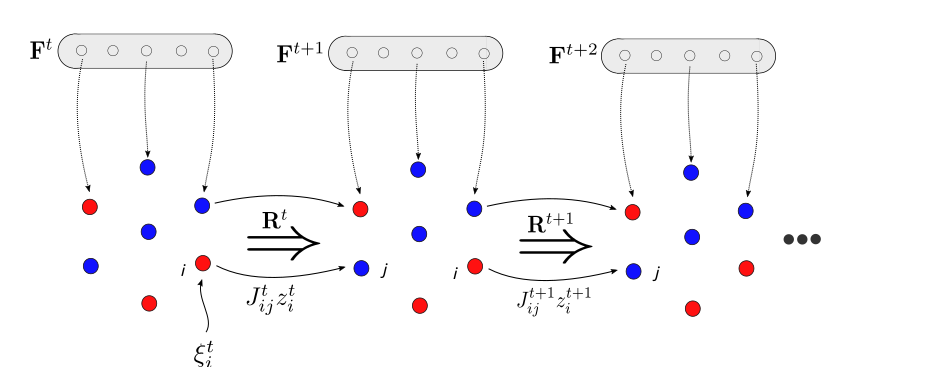
\includegraphics[width=150mm]{figure-1}
\caption{(a) Diagram of a recurrent neural network receving a time-dependent feedforward stimulus. (b) Diagram of the stochastic encoding scheme used a recurrent neural network with noise}
\end{figure}


\subsection{Synaptic plasticity and Bayesian models of cognition}

Synaptic plasticity refers to the activity-dependent modification of the strength or efficacy of synaptic transmission at preexisting synapses, and has been proposed to play a central role in the incorporation of transient experiences into persistent memory traces. The efficacy of an excitatory synapse can be either potentiated or depressed by a variety of mechanisms which occur over a wide range of time scales: from milliseconds to hours to days. Short-term synaptic plasticity (STP) is thought to play an important role in information processing in the brain. Its duration allows STP to modify the response of cortical circuits to stimuli and potentially provide a richer set of response properties without permanently altering the circuit architecture. One of several mechanisms thought to underly STP can be seen by the repeated stimulation of a presynaptic cell causing a transient accumulation of calcium in the presynaptic terminal (Mongillo et al. 2008). Calcium generally thought to elevate the probability of neurotransmitter release due to its proposed interaction with the biochemical machinery involved in synaptic vesicle excytosis. Other short term changes in synaptic efficacy can occur such as the facilitation or depression based upon the temporal characteristics of the stimulus. In paired-pulse experiments, a pair of stimuli is delivered a sub-20ms interval shows depression of the efficacy of the second stimulus (Zucker and Regehr, 2002). This phenomenon is hypothesized to arise from inactivation of voltage-dependent sodium and/or calcium channels or depletion of the release ready pool of synaptic vesicles at the presynaptic terminal [1]. Synaptic efficacy can be lowered by the release of biochemical modulators which can interact with the synaptic machinery to inhibit the release of neurotransmitter into the synaptic cleft. In addition, receptors at the presynaptic terminal which play a role in the secretion of neurotransmitter are sensitive to the presence of presynaptic neurmodulators. Therefore, these neuromodulators can also play a role in facilitation or depression in STP.

It is widely believed that neural circuits also possess the mechanisms for long term changes in synaptic strength formally referred to as long term potentiation (LTP) and long term depression (LTD). The brain encodes internally and externally generated stimuli as spatiotemporal patterns of action potentials and long-term modifications to such patterns via changes in synaptic transmission provide a feasible mechanism for the storage of information. In other words, changes in synaptic weights alter the spatiotemporal response of population of neurons to stimuli and therefore provide a method for long term memory formation. Since its original introduction by Cajal, this idea has been rigorously tested, for example in the CA1 region of the hippocampus (Whitlock et al. 2006). LTP and LTD have been extensively studied in the CA1 region of the hippocampus due to compelling evidence that it is a brain region that is central to learning and memory. Indeed, the cellular and biochemical mechanisms underlying these phenomena have been well-characterized. 


Significant effort has been spent in recent years to map the connectivity patterns of networks in cortex and thus variety of models have appeared. Connection patterns have been quantified by calculating a broad range of structural measures, including small-world attributes and motif composition, as well as some global measures of functional connectivity (Sporns 2006). The structural measures defined in this framework have proven quite useful; however, many models are defined without consideration of the fact that cortical networks are embedded in real space. In principle these spatially-dependent connectivity patterns could be hidden in the topology of an arbitrary graph; however, in some cases it is more straightforward to interpret connectivity patterns in the spatial domain. For example, the connectivity in a 2D lattice of LIF neurons with local and global synaptic connections are readily understood in terms of distances in real space (Rosenbaum 2014). At the same time, theoretical models e.g., mean-field theories of network dynamics have relaxed the strong assumption that cortical networks are spatially homogeneous (Brunel 2000). Defining a periodic connectivity kernel for each neuron on a lattice is an attractive model for cortical networks as it allows us to explore the dynamical consequences of translational invariance.

From the perspective of dynamical systems, sensory processing is often interpreted as an attraction of the neural state variables to a particular state corresponding to the encoding of the sensory stimulus. This point of view adopts the notion that sensory stimuli are then represented in the brain by \emph{attractor states} or locations in phase space which the network is driven towards during sensory processing (Hopfield, 1982). Early models of this form were deterministic in that the path taken towards a fixed steady state of the network dynamics is entirely determined by the initial conditions. On the other hand, recent experimental evidence suggests that neurons, synapses, and neural systems are inherently stochastic (Buesing 2011). These observations have provoked a dramatic paradigm shift in the way we view computations as being carried out in the brain. Namely, researchers now widely believe that information processing by the brain is carried out via a form of probabilistic inference.

Variability in sensory stimuli and the biological constitution of networks of neurons require the brain to make inferences about the external world amidst uncertainty. For example, the perception of objects in the external world by an organism is, in part, the transformation of a noisy continously valued variable to a discrete mental representation of the object. The injection of stochasticity into the pathway mapping stimuli to their neural representation has led many to believe that networks of neurons represent probability distributions rather than implementing logical circuits. Interestingly, behavioral studies have confirmed that human observers not only take uncertainty into account in a wide variety of tasks, but do so in a way that is nearly optimal (Ma 2006). It stands to reason that variability in sensory stimuli and performing inference amidst uncertainty are two sides of the same coin. If sensory stimuli were not variable, meaning that the mapping of sensory stimuli to neural responses was deterministic, the neural response from trial to trial would be identical. Therefore, the ability to handle small variations in the stimulus and the ability to generalize would be diminished.

Probabilistic inference is a well-established mathematical framework for making logical conclusions when only partial information is given or when the full information has become corrupt. Indeed, this framework is a critical tool in modern machine learning and artificial intelligence. A typical inference scenario is the deduction of the probability that the observed information was drawn from a distribution already known by the model. That is, the encoding scheme during sensory processing is the distribution of responses conditioned on the stimulus i.e., the posterior distribution $P(R|S)$. In the context of biological and artificial neural networks, that distribution is often \emph{learned} by the model via previous exposure to a large number of samples from the so-called population distribution of the data or stimulus. However, the mechanism by which spiking neural networks carry out inference tasks remains unclear. 

A popular point of view is that neural activity can be expressed in discrete-time and the set of spikes in each time bin can be interpreted as samples from the posterior $P(R|S)$, a distribution which is encoded by the synaptic weights. This interpretation has spawned the development of interesting parallels between neural dynamics and statistical sampling processes such as Markov chain Monte Carlo (MCMC) sampling (Buesing 2011). However, the interpretation of neural dynamics as implementing an artificial sampling process as in the Boltzmann machine, necessarily excludes biological details, such as synaptic plasticity and spike-adaptation, which are thought to play a major role in neural computation.


\section{Results}


%\begin{sidewaysfigure}
%\centering
%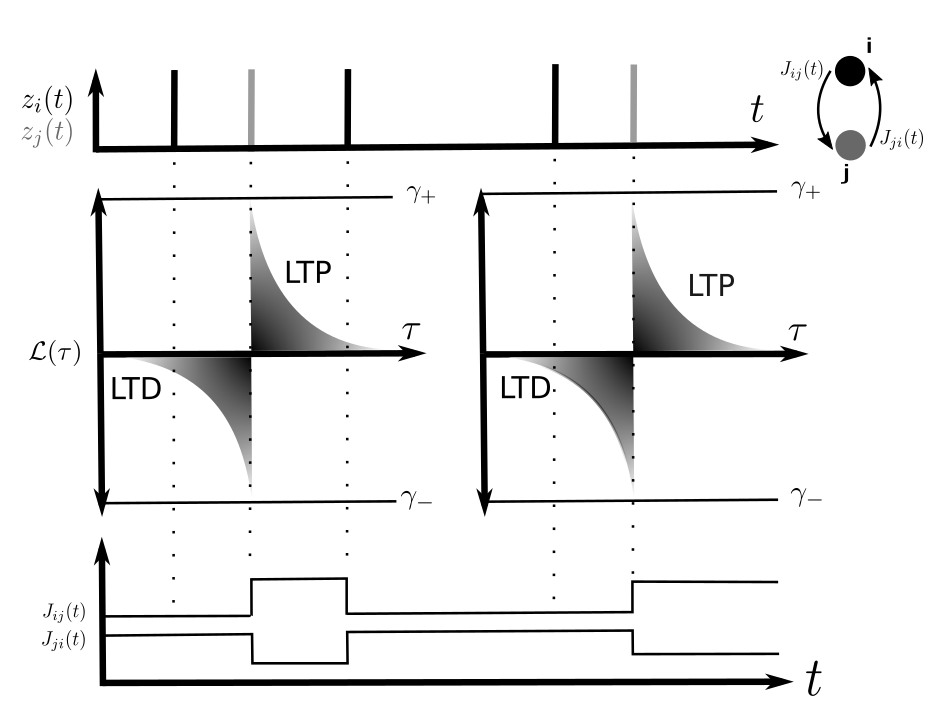
\includegraphics[scale=1.1]{figure-2}
%\caption{Weak correlations of synaptic currents in the asychronous state}
%\label{fig:foo}
%\end{sidewaysfigure}


\begin{figure}[t!]
\centering
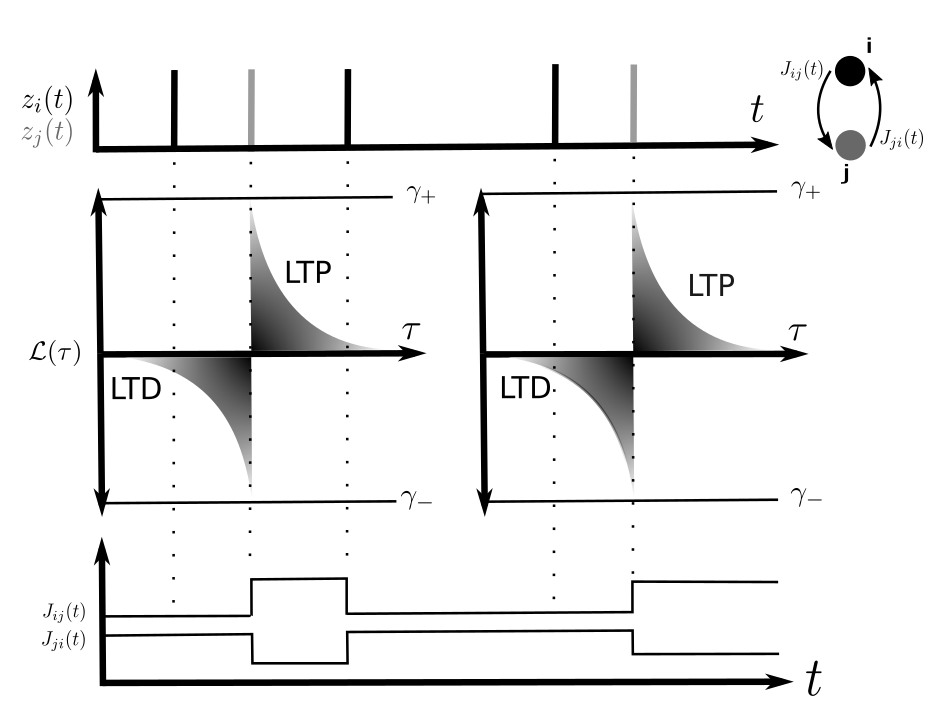
\includegraphics[width=175mm]{figure-2}
\caption{}
\end{figure}

\begin{figure}[t!]
\centering

\includegraphics[width=150mm]{figure-3}
\caption{}
\end{figure}



\section{Methods}


\subsection{Signal processing techniques}

The cross-correlation of discrete signals $x(t)$ and $y(t)$ is generally defined as the following convolution in the time-domain

\begin{align}
R_{xy}(\tau) = x(t) * y(t) = \sum_{k =-\infty}^{\infty}x(t)y(t+\tau)
\end{align}

where the $*$ symbol represents the convolution operation. Let $\psi_{x}(\omega)$ be the discrete-time Fourier transform (DTFT) of $x(t)$ i.e.,

\begin{align}
\psi_{x}(\omega) = \sum_{t =-\infty}^{\infty}x(t)\left(\exp{-i\omega t}\right)
\end{align}

where an identical expression exists for $\psi_{y}(\omega)$. According to the convolution theorem, convolution in the time-domain is equivalent to multiplication in the frequency domain with one of the signals time-reversed. Therefore, we can write

\begin{align}
\mathrm{DTFT}[x(t) * y(t)](\omega) = \underset{T\rightarrow\infty}{\mathrm{lim}}\frac{1}{2\pi T}\psi_{x}^{*}(\omega)\psi_{y}(\omega)
\end{align}


Let $S_{xy}(\omega) = \underset{T\rightarrow\infty}{\mathrm{lim}}\frac{1}{2\pi T}\psi_{x}^{*}(\omega)\psi_{y}(\omega)$, which is commonly called the \emph{cross spectral density} of signals $x(t)$ and $y(t)$. This is simply the DTFT of the cross-correlation function meaning that $R_{xx}(\tau)$ and $S_{xx}(\omega)$ form a Fourier pair. This result provides us an efficient means of computing cross-correlations and autocorrelations of synaptic currents by multiplication in the frequency domain and taking the inverse discrete transform.

\begin{appendices}
\end{appendices}

% Format a LaTeX bibliography
\makebibliography

[1] D.O. Hebb \textit{The organization of behavior: A neurophysiological theory}. John Wiley and Sons. 1949.

% Figures and tables, if you decide to leave them to the end
%\input{figure}
%\input{table}

\end{document}


